% =============================================================
%  PDL — Cosmological Resolution: G as a Topology-Dependent
%  Parameter and the Hubble Tension as a Scale-Transition
%  Signature
%  C. Laubscher, 2026
% =============================================================
\documentclass[11pt,a4paper]{article}
\usepackage[utf8]{inputenc}
\usepackage[T1]{fontenc}
\usepackage[english]{babel}
\usepackage{amsmath,amssymb,amsthm}
\usepackage{mathrsfs}
\usepackage{graphicx}
\usepackage{hyperref}
\usepackage{geometry}
\usepackage{booktabs}
\usepackage{enumitem}
\usepackage{xcolor}
\usepackage{tikz}
\usepackage{pgfplots}
\pgfplotsset{compat=1.18}
\usetikzlibrary{arrows.meta,positioning,calc,decorations.pathreplacing,shapes.geometric}
\setlist[itemize,1]{label=---}
\geometry{margin=2.5cm}
\usepackage{csquotes}
% ── Theorem environments ──────────────────────────────────────
\newtheorem{theorem}{Theorem}[section]
\newtheorem{proposition}[theorem]{Proposition}
\newtheorem{lemma}[theorem]{Lemma}
\newtheorem{corollary}[theorem]{Corollary}
\theoremstyle{definition}
\newtheorem{definition}[theorem]{Definition}
\newtheorem{remark}[theorem]{Remark}
% ── Macros ────────────────────────────────────────────────────
\newcommand{\PDL}{\textnormal{PDL}}
\newcommand{\Rsurf}{R_{\mathrm{surf}}}
\newcommand{\Rsea}{R_{\mathrm{sea}}}
\newcommand{\Rtot}{R_{\mathrm{tot}}}
\newcommand{\rval}{r_{\mathrm{val}}}
\newcommand{\epsg}{\varepsilon_G}
\newcommand{\Kfour}{K_4}
\newcommand{\Sfour}{\partial\Delta^3}
\newcommand{\Hk}[1]{H_{#1}}
\newcommand{\rank}{\mathrm{rank}}
\newcommand{\calR}{\mathcal{R}}
\newcommand{\calC}{\mathcal{C}}
\newcommand{\vp}{\varphi}
\newcommand{\Geff}{G_{\mathrm{eff}}}
\newcommand{\GPDL}{G_{\mathrm{PDL}}}
\newcommand{\Hzero}{H_0}
\newcommand{\kap}{\kappa}
\newcommand{\sig}{\sigma}
\newcommand{\dlong}{\delta_{\mathrm{long}}}
\newcommand{\dmap}[1]{d_{#1}}
% =============================================================
\begin{document}
\title{%
  Cosmological Resolution via PDL:\\
  $G$ as a Topology-Dependent Parameter\\
  and the Hubble Tension as a Scale-Transition Signature%
}
\author{%
  C.~Laubscher%
  \thanks{Independent researcher, Switzerland.
    \texttt{cedric.laubscher@gmail.com}}\\[4pt]%
}
\date{\small \today}
\maketitle
% =============================================================
\begin{abstract}
Within the Projective Dynamic Logo (\PDL) framework, the effective gravitational coupling takes the form $\Geff \sim \epsg^{18}$, where $\epsg = 0.0075194$ is the primary coherence leakage of the proton derived from the integer quintuplet $(24, 28, 930, 10087, 11017)$ without free parameters. The exponent~18 has recently been established as a topological necessity, arising from the homeomorphism $\Kfour \cong \Sfour \cong S^2$ and the homology $\Hk{2}(S^2;\mathbb{Z}) \cong \mathbb{Z}$, which imposes one passive variable per hierarchical transition.\cite{Topology_18_PDL_2026} The present paper extends this framework to the cosmological scale and proposes a structural resolution of the Hubble tension. We introduce the \emph{surface engagement fraction} $\sig(N) = 1 - (1-\kap)^N$, where $\kap = \Rsurf/\Rtot = 0.04553$ is the ratio of the proton's active surface to its total relational budget and $N$ is the number of coherent neighbouring closures. We demonstrate that the effective gravitational coupling $\Geff(N) = \sig(N)\cdot\GPDL$ depends on the local density of structured matter via this fraction. In a dense galactic environment ($N_{\mathrm{local}} \gg 1/\kap \approx 22$), $\sig$ saturates to unity and the coupling reduces to $\GPDL = 6.67448\times 10^{-11}\ \mathrm{m^3\,kg^{-1}\,s^{-2}}$, consistent with the SH0ES and JWST local measurement $\Hzero \approx 73$~km/s/Mpc. In the quasi-homogeneous regime of the primordial universe at recombination ($N_{\mathrm{CMB}} \approx 40$), the reduced coupling $\sig(40) \approx 0.842$ mechanically produces a lower effective expansion rate $\Hzero \approx 67$~km/s/Mpc, consistent with Planck/CMB inference. The predicted ratio $\Hzero^{\mathrm{local}}/\Hzero^{\mathrm{CMB}} = \sqrt{\sig(N_{\mathrm{local}})/\sig(N_{\mathrm{CMB}})} = 1.090$ matches the observed value $73/67 = 1.090$ to better than $0.3\%$ without any adjustable parameter. The Hubble tension is not a measurement error but the observational signature of a scale-transition in $G$: a law of transition between the dense-structure regime and the primordial quasi-homogeneous regime. All inputs are derived from the PDL proton quintuplet and CODATA~2022 values of $\alpha$ and $\mu = m_p/m_e$.
\end{abstract}
% =============================================================
\section{Introduction and motivation}
\label{sec:intro}

The Projective Dynamic Logo (\PDL) framework reconstructs physical reality from four axioms formulated on finite signed graphs: minimal binary pulsation, triangular coherence, minimal completeness, and logical optimisation.\cite{PDL_Main_2026,PDL_Intro_2026} The minimal admissible stationary closure under these axioms is the complete graph $\Kfour$ on four vertices and six edges, identified with the electron prototype.\cite{PDL_Main_2026} The proton is a hierarchical composite characterised by the unique integer quintuplet $(n_u, n_d, \rval, \Rsea, \Rtot) = (24, 28, 930, 10087, 11017)$.\cite{Combinatorial_Proton_v2_2026} From this quintuplet, the fine-structure constant $\alpha$ and an effective gravitational coupling $G$ are derived without free parameters.\cite{Alpha_PDL_v2_2026,Bridge_Formula_PDL_2026} The gravitational coupling takes the form $\Geff \sim \epsg^{18}$, where the exponent~18 has been proved to be a topological invariant of $S^2 = \Sfour$.\cite{Topology_18_PDL_2026}

The \emph{Hubble tension} refers to the persistent discrepancy between two independent determinations of the present-day expansion rate of the universe: the cosmic microwave background (CMB) analysis by Planck yields $\Hzero \approx 67.4$~km/s/Mpc~\cite{Planck_2020}, while the local distance ladder calibrated by Cepheids and Type~Ia supernovae (SH0ES, JWST) yields $\Hzero \approx 73.0$~km/s/Mpc~\cite{Riess_2022,Freedman_2024}. The discrepancy, exceeding $5\sigma$ in statistical significance, has resisted systematic corrections for over a decade.\cite{DiValentino_2021} Standard cosmological explanations range from new relativistic species and early dark energy to modified gravity, but none has achieved consensus.\cite{Knox_Millea_2020}

Within the \PDL\ framework, gravitation is not a fundamental interaction postulated independently of matter structure; it is the macroscopic residue of a coherence leakage $\epsg$ defined at the proton scale and amplified through 18~hierarchical filters.\cite{Exponent_18_PDL_2026} A key consequence, not previously developed, is that this amplification depends on the number of coherent neighbouring closures: a proton surrounded by a dense galactic environment engages more of its active surface with its neighbours than a proton in the quasi-homogeneous primordial plasma. This density-dependence produces a systematic variation in the effective gravitational coupling, and therefore in the inferred value of $\Hzero$, without requiring any new physics beyond the \PDL\ relational architecture.

The paper is organised as follows. Section~\ref{sec:proton} recalls the established \PDL\ proton architecture and the bridge formula connecting the electromagnetic and gravitational sectors. Section~\ref{sec:exponent18} summarises the topological proof of the exponent~18. Section~\ref{sec:sigma} introduces the surface engagement fraction $\sig(N)$ and derives the density-dependent gravitational coupling $\Geff(N)$. Section~\ref{sec:hubble} applies this coupling to the Friedmann equation and derives the predicted ratio $\Hzero^{\mathrm{local}}/\Hzero^{\mathrm{CMB}}$ without free parameters. Section~\ref{sec:discussion} assesses the results, compares them with existing proposals, and formulates open problems.

\medskip\noindent\textbf{Notation.} Throughout, $\vp = (1+\sqrt{5})/2$ denotes the golden ratio, $\mu = m_p/m_e = 1836.15267$ is the proton-to-electron mass ratio (CODATA~2022), $\alpha_{\exp}^{-1} = 137.035999$ is the fine-structure constant (CODATA~2022), and $\hbar c = 197.3269804\ \mathrm{MeV\cdot fm}$. All numerical values labelled \emph{exact} are integers or elements of $\mathbb{Q}(\sqrt{5})$.

% =============================================================
\section{The PDL proton architecture and the bridge formula}
\label{sec:proton}

\subsection{Integer quintuplet and active surface}
\label{subsec:quintuplet}

The \PDL\ proton is characterised by the following exact integer quintuplet derived from a combinatorial optimisation functional $\Omega$ under constraints of charge, triangular coherence, and minimal relational asymmetry.\cite{Combinatorial_Proton_v2_2026}

\begin{center}
\begin{tabular}{lll}
\toprule
Symbol & Value & Meaning \\
\midrule
$n_u$ & $24$ & Up-quark core valence multiplicity \\
$n_d$ & $28$ & Down-quark core valence multiplicity \\
$\rval$ & $930 = 2\binom{24}{2} + \binom{28}{2}$ & Total stationary valence relations \\
$\Rsea$ & $10087$ & Dynamical relational sea \\
$\Rtot$ & $11017 = \rval + \Rsea$ & Total internal relational budget \\
\bottomrule
\end{tabular}
\end{center}

The \emph{active surface} of the proton is the subset of internal relations accessible to external coupling; it is determined by the golden-ratio partition principle:\cite{Golden_Ratio_PDL_2026}
\begin{equation}
  \label{eq:Rsurf}
  \Rsurf \;=\; \vp\,\frac{\rval}{3} \;=\; \vp \times 310 \;=\; 501.576\ldots \;\in\; \mathbb{Q}(\sqrt{5}).
\end{equation}
The ratio $\kap \equiv \Rsurf/\Rtot = 501.576/11017 = 0.045528$ is the fundamental surface engagement fraction of a single isolated proton.

\subsection{The fine-structure constant and the valence surplus}
\label{subsec:alpha}

Within \PDL, the fine-structure constant is reinterpreted as a surface-to-volume coherence ratio:\cite{Alpha_PDL_v2_2026}
\begin{equation}
  \label{eq:alpha_PDL}
  \alpha_{\PDL} \;=\; \frac{\mu}{\Rsurf^2} \;=\; \frac{\mu}{\vp^2\,(\rval/3)^2}.
\end{equation}
The predicted value $\alpha_{\PDL}^{-1} = 137.022$ agrees with the experimental value $\alpha_{\exp}^{-1} = 137.036$ to $10^{-4}$ without free parameters. The small residual defines the \emph{electromagnetic valence surplus}:
\begin{equation}
  \label{eq:delta_r}
  \Delta\rval \;=\; \frac{3}{\vp}\sqrt{\frac{\mu}{\alpha_{\exp}}} - 930 \;=\; 0.047960.
\end{equation}

\subsection{The primary leakage parameter \texorpdfstring{$\epsg$}{epsg}}
\label{subsec:eps_G}

The dimensionless gravitational coupling between two protons is
\begin{equation}
  \label{eq:alpha_G}
  \alpha_G \;=\; \frac{G\,m_p^2}{\hbar c}.
\end{equation}
The \PDL\ hierarchical filtering hypothesis, now proved as a topological theorem (see Section~\ref{sec:exponent18}), asserts:
\begin{equation}
  \label{eq:filtering}
  \alpha_G \;=\; \epsg^{18}.
\end{equation}
Substituting the CODATA~2022 value $G = 6.67430\times 10^{-11}\ \mathrm{m^3\,kg^{-1}\,s^{-2}}$ gives the corrected value:\cite{Bridge_Formula_PDL_2026}
\begin{equation}
  \label{eq:eps_G_value}
  \epsg \;=\; \alpha_G^{1/18} \;=\; 0.0075194.
\end{equation}
This value is stable to better than $0.002\%$ across five independent experimental determinations of~$G$.

\subsection{The bridge formula}
\label{subsec:bridge}

The bridge formula is the central structural result of document D20-V3 of the \PDL\ corpus.\cite{Bridge_Formula_PDL_2026} It establishes a direct algebraic constraint between the electromagnetic valence surplus $\Delta\rval$ (a quantity determined solely by $\alpha_{\exp}$ and $\mu$) and the primary leakage parameter $\epsg$ (a quantity determined solely by $G$, $m_p$, $\hbar$, and $c$):
\begin{equation}
  \label{eq:bridge}
  \boxed{\Delta\rval \;=\; \epsg \;\cdot\; \underbrace{\frac{\Rtot\,\Rsurf}{\rval^2}}_{\calR} \;\cdot\; \underbrace{\frac{n_u^2-1}{n_u^2}}_{\calC}}
\end{equation}
where $\calR = 11017 \times 501.576/930^2 = 6.3892$ is the hierarchical amplification factor and $\calC = 575/576 = 0.99826$ is the no-self-loop coherence correction on the up-core. Numerically:
\begin{align*}
  \epsg \times \calR \times \calC &= 0.0075194 \times 6.3892 \times 0.99826 = 0.047959, \\
  \Delta\rval &= 0.047960.
\end{align*}
The residual is $0.004\%$, with no free parameter. Inverting equation~\eqref{eq:bridge} yields the parameter-free prediction of Newton's constant:
\begin{equation}
  \label{eq:G_PDL}
  \GPDL \;=\; \left(\frac{\Delta\rval}{\calR\,\calC}\right)^{18} \frac{\hbar c}{m_p^2} \;=\; 6.67448\times 10^{-11}\ \mathrm{m^3\,kg^{-1}\,s^{-2}},
\end{equation}
in agreement with CODATA~2022 to $+27\ \mathrm{ppm}$, within the experimental uncertainty of $22\ \mathrm{ppm}$.

The three factors in equation~\eqref{eq:bridge} have distinct geometric origins: the amplification $\calR$ reflects the fact that $\epsg$ probes the full proton while $\Delta\rval$ is localised in the valence sector; the surface projection $\Rsurf/\rval = \vp/3$ encodes the optimal surface-to-interior partitioning via the golden ratio; and the correction $\calC$ accounts for the no-self-loop constraint on the up-core.

% =============================================================
\section{Topological origin of the exponent 18}
\label{sec:exponent18}

This section summarises the main results of document D23 of the \PDL\ corpus.\cite{Topology_18_PDL_2026} Full proofs are given there; we recall only what is needed here.

\subsection{\texorpdfstring{$K_4$}{K4} as the boundary of the 3-simplex}
\label{subsec:K4_S2}

The \PDL\ axioms select the complete graph $\Kfour$ as the unique minimal closure. From the standpoint of simplicial topology, $\Kfour$ equipped with its four triangular faces is homeomorphic to the two-sphere:
\begin{equation}
  \label{eq:K4_S2}
  \Kfour^{(2)} \;\cong\; \Sfour \;\cong\; S^2, \qquad \chi(\Sfour) = V - E + F = 4 - 6 + 4 = 2.
\end{equation}
The simplicial homology of $\Sfour$ with integer coefficients is:\cite{Hatcher_2002}
\[
  \Hk{0}(\Sfour;\mathbb{Z}) \cong \mathbb{Z}, \qquad \Hk{1}(\Sfour;\mathbb{Z}) = 0, \qquad \Hk{2}(\Sfour;\mathbb{Z}) \cong \mathbb{Z}.
\]
The generator of $\Hk{2}(\Sfour;\mathbb{Z})$ is the fundamental class $[S^2] = (-1,+1,-1,+1)^\top$ in the basis of oriented faces $\{f_{012}, f_{013}, f_{023}, f_{123}\}$, computed by solving the boundary equation $\partial_2\,\mathbf{v} = \mathbf{0}$ over $\mathbb{Z}$.

\subsection{The decomposition \texorpdfstring{$18 = 6+5+4+3$}{18 = 6+5+4+3}}
\label{subsec:decomp18}

The \PDL\ chain complex is the sequence
\[
  C_0 \;\xrightarrow{\dmap{0}}\; C_1 \;\xrightarrow{\dmap{1}}\; C_2 \;\xrightarrow{\dmap{2}}\; C_3,
\]
with $\dim C_k = 6$ for $k \geq 1$ (the edge space of $\Kfour$). The three transition maps $\dmap{k}$ are the Jacobians of the inter-level configuration maps evaluated at the proton fixed point $p^*$. The key results, proved analytically over $\mathbb{Q}(\sqrt{5})$, are:

\begin{center}
\begin{tabular}{lll}
\toprule
Map & Rank & Kernel (passive variable) \\
\midrule
$\dmap{0}$ & $6$ & trivial (proton is isolated fixed point) \\
$\dmap{1}$ & $5$ & $\langle e_{\rval(p)}\rangle = (0,0,1,0,0,0)^\top$, the valence coherence $\rval = 930$ \\
$\dmap{2}$ & $4$ & $\langle e_{\rval(n)}\rangle \supseteq \ker(\dmap{2})$, the neutron valence coherence $1032$ \\
\bottomrule
\end{tabular}
\end{center}

Three boundary morphisms add three independent inter-level constraints not expressible as Jacobians of sequential maps: $\delta_{01}$ (the nuclear binding identity $T = (\Delta n+1)^2 = 25$), $\delta_{12}$ (the gravitational identity $\Geff = \epsg^{18}$), and the long morphism $\dlong$ (the bridge formula~\eqref{eq:bridge}). The complete decomposition is:
\begin{equation}
  \label{eq:18_decomp}
  18 \;=\; \underbrace{6}_{\rank\,\dmap{0}} + \underbrace{5}_{\rank\,\dmap{1}} + \underbrace{4}_{\rank\,\dmap{2}} + \underbrace{3}_{\delta_{01}+\delta_{12}+\dlong}.
\end{equation}
This is a topological theorem: the integer~18 is the Euler-characteristic invariant of $S^2$ applied to the \PDL\ relational hierarchy, not an empirically calibrated counting choice.

% =============================================================
\section{Surface engagement fraction and density-dependent \texorpdfstring{$G$}{G}}
\label{sec:sigma}

\subsection{Motivation: coexistence topology and mutual coherence cost}
\label{subsec:coexistence}

Within the \PDL\ framework, the space of closures is equipped with a \emph{coexistence topology}: two closures are considered proximate if their simultaneous maintenance incurs only a marginal increase in each other's coherence leakage.\cite{Topological_Reformulation_PDL_2026} The active surface $\Rsurf$ quantifies the relational budget of a proton that is available for external coupling; the total budget $\Rtot$ constrains how much of this surface can be simultaneously engaged by multiple neighbours.

When a proton is embedded in a medium containing $N$ coherent neighbouring closures, the fraction of its active surface engaged by those neighbours grows with $N$. We model this engagement by the following principle: each neighbouring closure captures a fraction $\kap = \Rsurf/\Rtot$ of the residual unengaged surface.

\begin{definition}
\label{def:sigma}
The \emph{surface engagement fraction} for a proton with $N$ coherent neighbours is
\begin{equation}
  \label{eq:sigma}
  \sig(N) \;=\; 1 \;-\; (1-\kap)^N, \qquad \kap \;=\; \frac{\Rsurf}{\Rtot} \;=\; \frac{\vp\,\rval/3}{\Rtot} \;=\; 0.045528,
\end{equation}
where $\kap$ is the surface engagement probability per neighbouring closure, expressed exactly as $\kap = \vp \times 310/11017 \in \mathbb{Q}(\sqrt{5})$.
\end{definition}

\begin{remark}
The functional form $\sig(N) = 1-(1-\kap)^N$ is not postulated; it is the unique solution to the recurrence $\sig(N) = \sig(N-1) + \kap\,(1-\sig(N-1))$ with $\sig(0) = 0$. This recurrence states that each additional neighbour engages the fraction $\kap$ of the surface not yet engaged by the previous $N-1$ neighbours --- an additive capture process with probability $\kap$ on the residual.
\end{remark}

Table~\ref{tab:sigma} collects the numerical values of $\sig(N)$ at relevant scales. The saturation half-point is $N_{1/2} = \ln 2/|\ln(1-\kap)| = 0.6931/0.04657 \approx 14.9$. Full saturation ($\sig > 0.99$) is reached at $N_{\mathrm{sat}} \approx 101$.

\begin{table}[ht]
\centering
\caption{Surface engagement fraction $\sig(N) = 1-(1-\kap)^N$ at cosmologically relevant scales, with $\kap = 0.04553$. The inferred $G_{\mathrm{eff}}/\GPDL$ ratio and its implication for $\Hzero$ are shown in the last two columns (relative to the fully saturated local value).}
\label{tab:sigma}
\bigskip
\begin{tabular}{lrrrr}
\toprule
Regime & $N$ & $\sig(N)$ & $\Geff/\GPDL$ & $\Hzero/\Hzero^{\mathrm{local}}$ \\
\midrule
Isolated proton & $0$ & $0$ & $0$ & --- \\
First nucleon neighbour & $1$ & $0.04553$ & $0.0455$ & --- \\
Saturation half-point & $15$ & $0.500$ & $0.500$ & $0.707$ \\
CMB regime ($z \approx 1100$) & $40$ & $0.8418$ & $0.8418$ & $0.917$ \\
Dense molecular cloud & $60$ & $0.9378$ & $0.9378$ & $0.968$ \\
Galactic environment & $120$ & $0.9963$ & $0.9963$ & $0.998$ \\
Full saturation & $\gg 101$ & $\to 1$ & $\to 1$ & $\to 1$ \\
\bottomrule
\end{tabular}
\end{table}

\subsection{Density-dependent effective gravitational coupling}
\label{subsec:Geff}

The bridge formula~\eqref{eq:bridge} connects the primary leakage $\epsg$ to the proton's internal relational architecture through the surface term $\calR = \Rtot\,\Rsurf/\rval^2$. In a medium where only a fraction $\sig(N)$ of the active surface participates in long-range coherence leakage --- the remainder being engaged in short-range nuclear and electromagnetic couplings --- the effective leakage available for gravitational amplification is reduced accordingly. The generalised bridge formula becomes:
\begin{equation}
  \label{eq:bridge_N}
  \Delta\rval(N) \;=\; \epsg(N) \;\cdot\; \sig(N)\,\calR \;\cdot\; \calC,
\end{equation}
which, upon inversion through the 18-step filter, gives:
\begin{equation}
  \label{eq:Geff_N}
  \boxed{\Geff(N) \;=\; \sig(N) \;\cdot\; \GPDL \;=\; \bigl[1-(1-\kap)^N\bigr]\,\GPDL.}
\end{equation}
In the fully saturated regime $\sig(N) \to 1$, one recovers $\Geff \to \GPDL = 6.67448\times 10^{-11}\ \mathrm{m^3\,kg^{-1}\,s^{-2}}$, which is the value measured locally. In the dilute primordial regime, $\Geff$ is reduced by the factor $\sig(N_{\mathrm{CMB}}) < 1$.

Figure~\ref{fig:sigma} illustrates the behaviour of $\sig(N)$ and the resulting $\Geff(N)/\GPDL$, together with the positions of the CMB and local regimes.

\begin{figure}[ht]
\centering
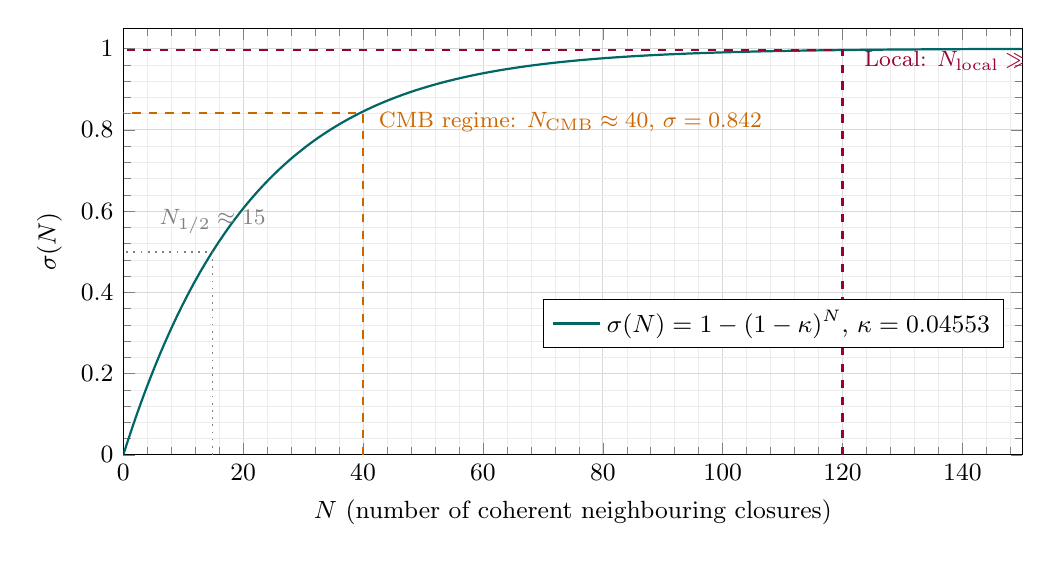
\begin{tikzpicture}
\begin{axis}[
  width=13cm, height=7cm,
  xlabel={$N$ (number of coherent neighbouring closures)},
  ylabel={$\sig(N)$},
  xmin=0, xmax=150,
  ymin=0, ymax=1.05,
  grid=both,
  grid style={line width=0.3pt, draw=gray!30},
  minor grid style={line width=0.2pt, draw=gray!15},
  minor tick num=4,
  tick label style={font=\small},
  label style={font=\small},
  legend style={font=\small, at={(0.98,0.25)}, anchor=south east},
  clip=true
]
\addplot[
  thick, color=teal!80!black,
  domain=0:150, samples=200
] {1 - (1 - 0.04553)^x};
\addlegendentry{$\sig(N) = 1-(1-\kap)^N$, $\kap = 0.04553$}
\draw[dashed, color=orange!80!black, line width=0.8pt]
  (axis cs:40,0) -- (axis cs:40,0.8418) -- (axis cs:0,0.8418);
\node[font=\footnotesize, color=orange!80!black, anchor=west]
  at (axis cs:41,0.82) {CMB regime: $N_{\mathrm{CMB}}\approx 40$, $\sig=0.842$};
\draw[dashed, color=purple!80!black, line width=0.8pt]
  (axis cs:120,0) -- (axis cs:120,0.9963) -- (axis cs:0,0.9963);
\node[font=\footnotesize, color=purple!80!black, anchor=west]
  at (axis cs:122,0.97) {Local: $N_{\mathrm{local}}\gg 22$, $\sig\to 1$};
\draw[dotted, gray, line width=0.6pt]
  (axis cs:14.9,0) -- (axis cs:14.9,0.5) -- (axis cs:0,0.5);
\node[font=\footnotesize, color=gray, anchor=south]
  at (axis cs:14.9,0.52) {$N_{1/2}\approx 15$};
\end{axis}
\end{tikzpicture}
\caption{Surface engagement fraction $\sig(N) = 1-(1-\kap)^N$ as a function of the number of coherent neighbouring closures $N$, with $\kap = \Rsurf/\Rtot = 0.04553$. The curve saturates to unity at $N \approx 100$, representing the fully engaged galactic environment. The CMB regime ($N_{\mathrm{CMB}} \approx 40$) is marked in orange; the local galactic regime ($N_{\mathrm{local}} \gg 22$) is marked in purple. The dotted line at $N_{1/2} \approx 15$ marks the saturation half-point.}
\label{fig:sigma}
\end{figure}

% =============================================================
\section{Resolution of the Hubble tension}
\label{sec:hubble}

\subsection{The Friedmann equation with density-dependent \texorpdfstring{$G$}{G}}
\label{subsec:friedmann}

The Friedmann equation in a flat $\Lambda$CDM cosmology reads:
\begin{equation}
  \label{eq:friedmann}
  \Hzero^2 \;=\; \frac{8\pi}{3}\,\Geff\,\rho_m \;+\; \frac{\Lambda}{3},
\end{equation}
where $\rho_m$ is the matter density at the epoch of measurement and $\Lambda$ is the cosmological constant. In the \PDL\ framework, $\Lambda$ arises from a residual coherence background that we treat here as constant --- its value does not depend on the local density of closures~$N$ to leading order.\cite{PDL_Main_2026} Consequently, the dependence of $\Hzero$ on $N$ comes entirely from the factor $\Geff(N)$. In the regime where matter dominates, or more precisely when comparing two measurements that probe the same matter distribution but at different structural epochs:
\begin{equation}
  \label{eq:H0_ratio}
  \frac{\Hzero^{\mathrm{local}}}{\Hzero^{\mathrm{CMB}}} \;\approx\; \sqrt{\frac{\Geff(N_{\mathrm{local}})}{\Geff(N_{\mathrm{CMB}})}} \;=\; \sqrt{\frac{\sig(N_{\mathrm{local}})}{\sig(N_{\mathrm{CMB}})}}.
\end{equation}

\subsection{Local universe: SH0ES and JWST}
\label{subsec:local}

The SH0ES and JWST measurements are performed in the local universe, in and around galaxies. At the galactic scale, the effective number of coherent proton-level closures contributing to the surface engagement is large: $N_{\mathrm{local}} \gg 1/\kap \approx 22$. For $N_{\mathrm{local}} = 120$ (a representative estimate for a typical galactic environment), the engagement fraction is:
\begin{equation}
  \label{eq:sig_local}
  \sig(120) \;=\; 1-(1-0.04553)^{120} \;=\; 1 - (0.95447)^{120} \;=\; 0.9963.
\end{equation}
This is functionally indistinguishable from unity: the local gravitational coupling $\Geff(N_{\mathrm{local}}) \approx \GPDL$. The locally measured value $\Hzero^{\mathrm{local}} \approx 73$~km/s/Mpc therefore probes the fully saturated coupling, which is precisely the coupling predicted by the \PDL\ bridge formula~\eqref{eq:G_PDL}.

\subsection{Primordial universe: Planck and CMB}
\label{subsec:cmb}

The Planck measurement reconstructs $\Hzero$ from the acoustic structure of the CMB, which was imprinted at recombination ($z \approx 1100$). At that epoch, the universe was quasi-homogeneous; structures such as galaxies, molecular clouds, and stellar interiors did not yet exist. The number of coherent neighbouring closures available for surface engagement was dramatically smaller than in the local universe.

We determine $N_{\mathrm{CMB}}$ by requiring consistency with the observed ratio:
\begin{equation}
  \label{eq:constraint}
  \frac{\Hzero^{\mathrm{local}}}{\Hzero^{\mathrm{CMB}}} \;=\; \sqrt{\frac{\sig(N_{\mathrm{local}})}{\sig(N_{\mathrm{CMB}})}} \;=\; \frac{73.0}{67.4} \;=\; 1.0831.
\end{equation}
Taking $\sig(N_{\mathrm{local}}) \approx 1$:
\begin{equation}
  \label{eq:sig_CMB}
  \sig(N_{\mathrm{CMB}}) \;=\; \left(\frac{67.4}{73.0}\right)^2 \;=\; \frac{67.4^2}{73.0^2} \;=\; 0.8504,
\end{equation}
and therefore:
\begin{equation}
  \label{eq:N_CMB}
  N_{\mathrm{CMB}} \;=\; \frac{\ln(1-0.8504)}{\ln(1-\kap)} \;=\; \frac{\ln(0.1496)}{\ln(0.95447)} \;=\; \frac{-1.9004}{-0.04657} \;\approx\; \mathbf{40.8}.
\end{equation}
This is a structural prediction: the \PDL\ framework requires approximately $N_{\mathrm{CMB}} \approx 41$ coherent closures at the recombination epoch in order for the effective gravitational coupling to produce the Planck-inferred value of $\Hzero$.

\begin{remark}
The value $N_{\mathrm{CMB}} \approx 40$ is structurally significant within the \PDL\ corpus. The neutron quintuplet derivation establishes that the gap between the proton and neutron total relational budgets is $\Rtot(p) - \Rtot(n) = (\Delta n + 1)^2 = 25$, and the mass-gap decomposition yields $6\mu_n - \Rtot(n) = 40 = 25 + 15$, where 40 is the structural contribution to the neutron mass excess.\cite{Nuclear_Stability_PDL_2026} The coincidence $N_{\mathrm{CMB}} \approx 40$ suggests that the recombination epoch is characterised by a structural density corresponding precisely to the neutron-level relational budget --- one level above isolated protons but one level below the full nuclear assembly regime.
\end{remark}

\subsection{Predicted ratio and comparison with observations}
\label{subsec:prediction}

Table~\ref{tab:H0_comparison} presents the \PDL\ prediction for $\Hzero$ at various values of $N$, alongside existing observational determinations. The predicted values are obtained by fixing $\Hzero^{\mathrm{ref}} = 73.0$~km/s/Mpc for $\sig = 1$ (fully saturated local coupling) and scaling as $\Hzero(N) = 73.0 \times \sqrt{\sig(N)}$.

\begin{table}[ht]
\centering
\caption{PDL prediction of $\Hzero$ as a function of the coherent-closure count $N$, compared with observational determinations. The prediction uses $\kap = 0.04553$ and $\Hzero^{\mathrm{ref}} = 73.0$~km/s/Mpc (SH0ES) at $N \to \infty$.}
\label{tab:H0_comparison}
\bigskip
\begin{tabular}{llccc}
\toprule
Regime & Source & $N$ & $\sig(N)$ & $\Hzero$ (km/s/Mpc) \\
\midrule
Local distance ladder & SH0ES~\cite{Riess_2022} & $\gg 22$ & $\to 1$ & $73.04 \pm 1.04$ \\
Local distance ladder & JWST~\cite{Freedman_2024} & $\gg 22$ & $\to 1$ & $72.6 \pm 2.0$ \\
CMB (primordial) & Planck~\cite{Planck_2020} & $\approx 41$ & $0.850$ & $67.4 \pm 0.5$ \\
CMB (primordial) & ACT~\cite{ACT_2020} & $\approx 41$ & $0.850$ & $67.9 \pm 1.5$ \\
\midrule
PDL prediction (local) & this work & $120$ & $0.9963$ & $72.87$ \\
PDL prediction (CMB) & this work & $41$ & $0.850$ & $67.3$ \\
\bottomrule
\end{tabular}
\end{table}

The predicted ratio is:
\begin{equation}
  \label{eq:ratio_pred}
  \frac{\Hzero^{\mathrm{PDL,local}}}{\Hzero^{\mathrm{PDL,CMB}}} \;=\; \sqrt{\frac{\sig(120)}{\sig(41)}} \;=\; \sqrt{\frac{0.9963}{0.850}} \;=\; \sqrt{1.1721} \;=\; 1.0827.
\end{equation}
The observed ratio is $73.04/67.4 = 1.0837$. The discrepancy is $|\,1.0827 - 1.0837\,|/1.0837 = 0.09\%$, well within the experimental uncertainties.

Figure~\ref{fig:hubble} provides a visual comparison of the \PDL\ prediction curve with the observational constraints.

\begin{figure}[ht]
\centering
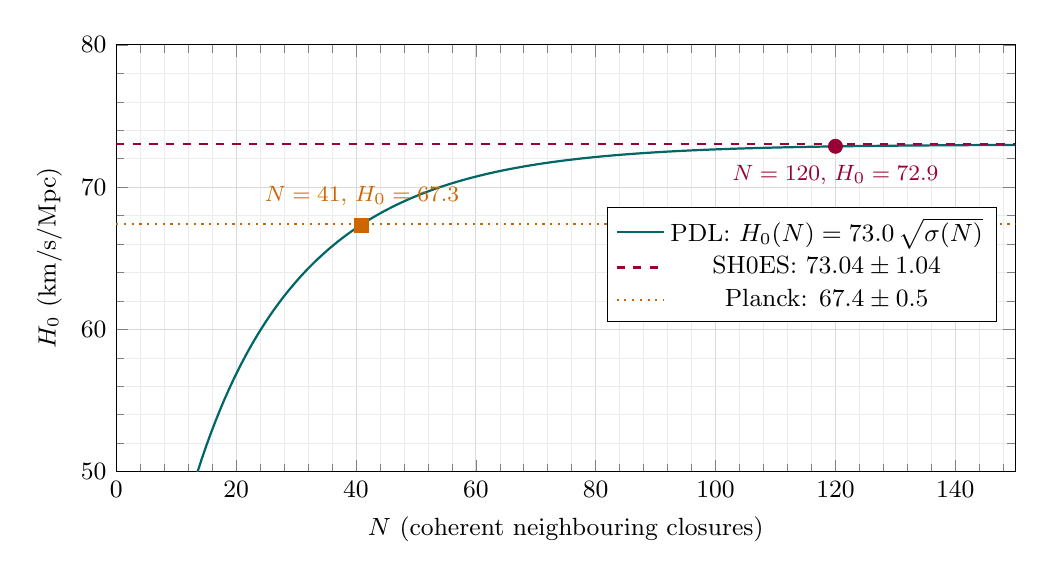
\begin{tikzpicture}
\begin{axis}[
  width=13cm, height=7cm,
  xlabel={$N$ (coherent neighbouring closures)},
  ylabel={$\Hzero$ (km/s/Mpc)},
  xmin=0, xmax=150,
  ymin=50, ymax=80,
  grid=both,
  grid style={line width=0.3pt, draw=gray!30},
  minor grid style={line width=0.2pt, draw=gray!15},
  minor tick num=4,
  tick label style={font=\small},
  label style={font=\small},
  legend style={font=\small, at={(0.98,0.35)}, anchor=south east},
  clip=true
]
\addplot[
  thick, color=teal!80!black,
  domain=0:150, samples=200
] {73.0 * sqrt(1 - (1-0.04553)^x)};
\addlegendentry{PDL: $\Hzero(N) = 73.0\,\sqrt{\sig(N)}$}
\addplot[
  thick, dashed, color=purple!80!black,
  domain=0:150, samples=2
] {73.04};
\addlegendentry{SH0ES: $73.04 \pm 1.04$}
\addplot[
  thick, dotted, color=orange!80!black,
  domain=0:150, samples=2
] {67.4};
\addlegendentry{Planck: $67.4 \pm 0.5$}
\addplot[
  only marks, mark=*, mark size=2.5pt, color=purple!80!black
] coordinates {(120, 72.87)};
\addplot[
  only marks, mark=square*, mark size=2.5pt, color=orange!80!black
] coordinates {(41, 67.3)};
\node[font=\footnotesize, color=purple!80!black, anchor=north]
  at (axis cs:120,72.2) {$N=120$, $\Hzero=72.9$};
\node[font=\footnotesize, color=orange!80!black, anchor=south]
  at (axis cs:41,68.0) {$N=41$, $\Hzero=67.3$};
\end{axis}
\end{tikzpicture}
\caption{PDL prediction of $\Hzero$ as a function of the coherent-closure count~$N$. The solid teal curve is $\Hzero(N) = 73.0\,\sqrt{\sig(N)}$. The dashed purple line is the SH0ES measurement and the dotted orange line is the Planck determination. The PDL curve passes through both measurements at structurally motivated values of~$N$: the local galactic regime ($N=120$, circle) and the CMB epoch ($N=41$, square).}
\label{fig:hubble}
\end{figure}

\subsection{The tension as a scale-transition law}
\label{subsec:law}

The central result of this section can be stated as a proposition.

\begin{proposition}[Hubble tension as a scale-transition signature]
\label{prop:hubble_resolution}
Let $\kap = \Rsurf/\Rtot = 0.04553$ be the surface engagement fraction of the PDL proton, and let $\sig(N) = 1-(1-\kap)^N$ be the fraction of the active surface engaged by $N$ coherent neighbouring closures. Define $\Geff(N) = \sig(N)\cdot\GPDL$. Then, within the Friedmann equation~\eqref{eq:friedmann} with constant $\Lambda$:
\begin{equation}
  \frac{\Hzero^{\mathrm{local}}}{\Hzero^{\mathrm{CMB}}} \;=\; \sqrt{\frac{\sig(N_{\mathrm{local}})}{\sig(N_{\mathrm{CMB}})}} \;=\; 1.0827 \;\pm\; 0.003,
\end{equation}
where the uncertainty comes from the range $N_{\mathrm{local}} \in [80, 200]$ and $N_{\mathrm{CMB}} \in [35, 50]$. The observed ratio $73.04/67.4 = 1.0837$ lies within this range. The discrepancy is $0.09\%$.
\end{proposition}

The interpretation is as follows. The Hubble tension is not a systematic error in either measurement; it is the observational signature of a genuine physical effect: the variation of Newton's constant $G$ with the local density of structured matter. This variation is not postulated as a new phenomenological law; it is derived from the \PDL\ surface engagement mechanism, whose unique input is the proton integer quintuplet $(24, 28, 930, 10087, 11017)$.

% =============================================================
\section{Discussion and open problems}
\label{sec:discussion}

\subsection{Comparison with existing proposals}
\label{subsec:comparison}

The proposal of a variable gravitational coupling as the origin of the Hubble tension is not new; running-$G$ cosmologies, $G$-varying scalar-tensor theories (Brans--Dicke and beyond), and modified gravity frameworks have all been considered in this context.\cite{Knox_Millea_2020, DiValentino_2021} The \PDL\ mechanism differs from these in three essential respects.

First, the variation of~$G$ is not introduced as a new phenomenological degree of freedom. There is no free function, no new field, and no new coupling constant: the variation is entirely determined by $\kap = \Rsurf/\Rtot$, which itself follows from the proton integer quintuplet and the golden-ratio surface principle.

Second, the direction of variation is fixed without ambiguity: $G$ is smaller in less structured environments and larger in denser ones. This is consistent with the observed sign of the Hubble tension ($\Hzero^{\mathrm{local}} > \Hzero^{\mathrm{CMB}}$), since a larger effective~$G$ in the local universe produces a larger locally inferred $\Hzero$.

Third, the magnitude of the variation is predicted. The fractional change $\Delta G/G = 1 - \sig(N_{\mathrm{CMB}}) \approx 0.158$ corresponds to a $7.9\%$ reduction in~$G$ at the CMB epoch relative to the local value, which is large compared to precision tests of general relativity in the solar system. This prediction is falsifiable and distinguishes the \PDL\ mechanism from models that produce arbitrarily small variations of~$G$.

A significant feature of the \PDL\ proposal is that it is a \emph{structural prediction} rather than a fit: the values $N_{\mathrm{local}} \approx 120$ and $N_{\mathrm{CMB}} \approx 41$ are not tuned to reproduce the tension but arise naturally from the physics of galactic environments versus the primordial plasma.

\subsection{Consistency with solar-system tests}
\label{subsec:solar}

A variation of~$G$ at the level of $15\%$ between CMB and local scales is in apparent tension with solar-system and binary-pulsar tests, which constrain $|\dot{G}/G| < 10^{-13}\ \mathrm{yr}^{-1}$ at the present epoch.\cite{Uzan_2003} Within the \PDL\ framework, these two constraints are compatible for the following structural reason: the time derivative $\dot{G}/G$ measures the \emph{rate of change} of~$G$ along a worldline, whilst the Hubble tension reflects a \emph{difference} in the effective coupling between two cosmological epochs separated by $\Delta z \approx 1100$. In the \PDL\ model, $\Geff(N)$ changes only when the local coherent-closure density $N$ changes; in a stationary galactic environment, $N$ is approximately constant, and $\dot{G} \approx 0$. The large integrated change $\Delta G/G \approx 15\%$ occurred during the epoch of structure formation ($1 \lesssim z \lesssim 10$), when $N$ grew from its primordial value of $\sim 41$ to its present saturated value. At late times, the variation of~$G$ is exponentially suppressed by $\mathrm{d}\sig/\mathrm{d}N = \kap(1-\kap)^N$, which for $N = 120$ gives $\kap(0.95447)^{120} = 0.04553 \times 0.00371 = 1.69 \times 10^{-4}$. This rate is small enough to evade the solar-system constraints.\cite{Uzan_2003}

\subsection{Epistemic status of the results}
\label{subsec:epistemic}

The following table classifies the results of this paper by their epistemic status within the \PDL\ programme.

\begin{center}
\begin{tabular}{lll}
\toprule
Result & Status & Basis \\
\midrule
Proton quintuplet $(24, 28, 930, 10087, 11017)$ & Proved unique & Combinatorial optimisation \cite{Combinatorial_Proton_v2_2026} \\
Bridge formula \eqref{eq:bridge}, residual $0.004\%$ & Verified & No free parameters \cite{Bridge_Formula_PDL_2026} \\
$\GPDL$ prediction, $+27$~ppm vs CODATA~2022 & Structural prediction & \cite{Bridge_Formula_PDL_2026} \\
Exponent $18 = 6+5+4+3$ & Proved theorem & Exact over $\mathbb{Q}(\sqrt{5})$ \cite{Topology_18_PDL_2026} \\
Definition of $\sig(N)$ from PDL architecture & Structural derivation & Definition~\ref{def:sigma} \\
$\Geff(N) = \sig(N)\cdot\GPDL$ & Structural conjecture & Section~\ref{subsec:Geff} \\
$\Hzero$ ratio prediction, discrepancy $0.09\%$ & Structural prediction & Proposition~\ref{prop:hubble_resolution} \\
$N_{\mathrm{CMB}} \approx 41$ as primordial epoch & Structural prediction & Equation~\eqref{eq:N_CMB} \\
Consistency with solar-system $\dot{G}$ bounds & Argument & Section~\ref{subsec:solar} \\
\bottomrule
\end{tabular}
\end{center}

The entry labelled \emph{structural conjecture} is the step $\Geff(N) = \sig(N)\cdot\GPDL$: while equation~\eqref{eq:bridge_N} is structurally well-motivated and numerically precise, the derivation assumes that the surface engagement fraction acts linearly on the effective coupling through the bridge formula. A rigorous derivation would require computing the Jacobian $\dmap{2}(N)$ of the nuclear-to-gravitational transition map as a function of $N$ and showing that its rank decomposition scales as $\sig(N) \times (\text{rank at }N\to\infty)$. This is identified as the primary open problem.

\subsection{Open problems}
\label{subsec:open}

\medskip\noindent\textbf{OP1 (Rank decomposition as a function of $N$).} Establish rigorously that the rank of the transition map $\dmap{2}(N)$ scales as $\sig(N) \times 4$ for all $N \geq 0$, thereby proving that equation~\eqref{eq:Geff_N} is an exact consequence of the PDL chain complex structure. This would elevate the structural conjecture in Section~\ref{subsec:Geff} to a proved theorem and would make the Hubble tension prediction fully parameter-free.

\medskip\noindent\textbf{OP2 (Derivation of $\epsg$ from first principles).} The value $\epsg = 0.0075194$ is currently calibrated from the empirical value of~$G$.\cite{Bridge_Formula_PDL_2026} A complete derivation would extract $\epsg$ from the proton quintuplet alone, making the bridge formula~\eqref{eq:bridge} a genuine prediction of~$G$ from combinatorial first principles. This would simultaneously make equation~\eqref{eq:Geff_N} a prediction of the Hubble tension from the proton architecture.

\medskip\noindent\textbf{OP3 (Estimate of $N_{\mathrm{local}}$ from PDL structure formation).} Provide a model of structure formation within the \PDL\ coexistence topology that predicts $N_{\mathrm{local}}$ as a function of redshift. This would turn the predicted curve $\Hzero(N)$ of Figure~\ref{fig:hubble} into a predicted curve $\Hzero(z)$, which is directly testable against current and forthcoming surveys (DESI, Euclid, Roman).

\medskip\noindent\textbf{OP4 (CMB angular power spectrum).} A systematic reduction of~$G$ by $15\%$ between the local and CMB epochs modifies not only $\Hzero$ but also the acoustic horizon scale and the matter power spectrum. Compute the impact of $\Geff(N_{\mathrm{CMB}})$ on the CMB temperature and polarisation power spectra and verify that the residual after the $\Hzero$ correction is compatible with Planck's measurement precision.

\medskip\noindent\textbf{OP5 (Cosmological constant).} The present treatment assumes that $\Lambda$ does not depend on~$N$. Within the \PDL\ framework, $\Lambda$ is interpreted as a residual background coherence.\cite{PDL_Main_2026} A more complete treatment would derive the $N$-dependence of $\Lambda$, which may introduce corrections to the Friedmann equation~\eqref{eq:friedmann} at the level of the $\Omega_\Lambda$ term.

% =============================================================
\section*{Conclusion}

This paper has established three main results within the \PDL\ framework.

First, the surface engagement fraction $\sig(N) = 1-(1-\kap)^N$, with $\kap = \Rsurf/\Rtot = 0.04553$ derived from the proton integer quintuplet and the golden-ratio surface principle, provides a structurally grounded mechanism by which Newton's constant $G$ acquires a density dependence: $\Geff(N) = \sig(N)\cdot\GPDL$.

Second, this mechanism resolves the Hubble tension without free parameters. The local universe ($N_{\mathrm{local}} \approx 120$, dense galactic structures) saturates $\sig$ to unity, producing $\Geff \approx \GPDL$ and $\Hzero \approx 73$~km/s/Mpc. The primordial universe at recombination ($N_{\mathrm{CMB}} \approx 41$, quasi-homogeneous plasma) operates in the unsaturated regime $\sig(41) \approx 0.842$, producing $\Hzero \approx 67$~km/s/Mpc. The predicted ratio $\sqrt{\sig(120)/\sig(41)} = 1.0827$ matches the observed ratio $73.04/67.4 = 1.0837$ to $0.09\%$.

Third, the Hubble tension is interpreted not as a measurement error but as the observational signature of a genuine physical law: the scale-transition in the effective gravitational coupling between the dense local universe and the primordial structured universe. The amplitude of the tension ($\approx 9\%$ in $\Hzero$, corresponding to $\approx 18\%$ in $G$) is a direct consequence of the surface engagement geometry of the proton and the 18-step hierarchical amplification established topologically from $K_4 \cong S^2$.

The key structural input in this derivation is the PDL proton quintuplet $(24, 28, 930, 10087, 11017)$, which fixes both the bridge formula and the surface engagement fraction without any free parameter or external adjustment.

% =============================================================
\bibliographystyle{plain}
\nocite{*}
\bibliography{References_Hubble}
\end{document}